\section{Theoretical Models}

\subsection{Capital Asset Pricing Model (CAPM)}
The Capital Asset Pricing Model (CAPM) is employed to determine the expected return on an asset based on its systematic risk, as measured by beta ($\beta_i$). The CAPM formula is:

\begin{equation}
E(R_i) = R_f + \beta_i(E(R_m) - R_f)
\end{equation}

\subsubsection{Beta Calculation}
Beta ($\beta_i$) measures the volatility of an asset in relation to the market. It is calculated as:
\begin{equation}
\beta_i = \frac{Cov(R_i, R_m)}{\sigma^2_m}
\end{equation}

\subsubsection{Security Market Line (SML)}
The Security Market Line (SML) is a graphical representation of the CAPM, showcasing the relationship between the expected return of an asset and its systematic risk, as measured by beta ($\beta_i$).

\begin{figure}[h!]
    \centering
    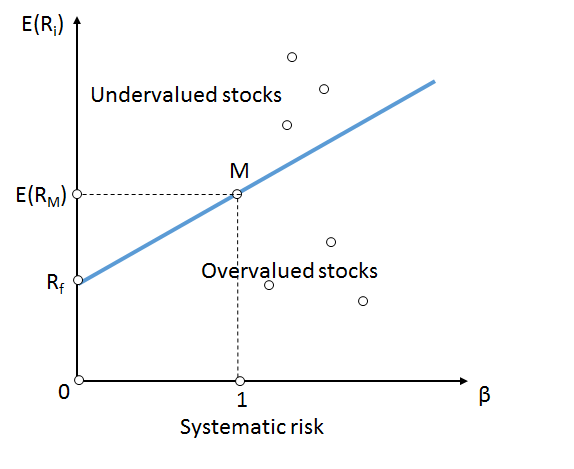
\includegraphics[width=0.6\textwidth]{../Figures/SML.png}
    \caption{Security Market Line}
    \label{fig:SML}
\end{figure}

\subsubsection{Theoretical Implications}
The SML conveys several important theoretical implications:
\begin{itemize}
    \item All securities, when correctly priced, should lie on the SML.
    \item The slope of the SML is the market risk premium, $E(R_m) - R_f$, representing the additional return expected from holding a market portfolio instead of risk-free assets.
    \item The intercept of the SML is the risk-free rate, $R_f$, reflecting the return of a theoretically risk-free asset.
\end{itemize}

\subsection{Modern Portfolio Theory (MPT)}
Modern Portfolio Theory provides a robust framework for constructing an optimal portfolio that maximizes expected return for a given level of risk. The expected return $E(R_p)$ of a portfolio is the weighted sum of the expected returns of the individual assets:
\begin{equation}
E(R_p) = \sum_{i=1}^n w_iE(R_i)
\end{equation}

\subsubsection{Efficient Frontier and Optimal Portfolio}
The efficient frontier is a concept from MPT that represents the set of optimal portfolios offering the highest expected return for a defined level of risk. The process of constructing the efficient frontier involves solving the following optimization problem:

\begin{equation}
\min \sum_{i=1}^n \sum_{j=1}^n w_i w_j \sigma_{ij}
\end{equation}

subject to:

\begin{equation}
\sum_{i=1}^n w_i = 1
\end{equation}

and

\begin{equation}
E(R_p) = \sum_{i=1}^n w_iE(R_i)
\end{equation}

\begin{figure}[h!]
    \centering
    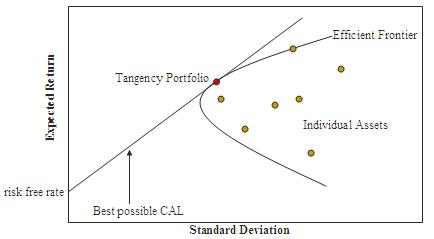
\includegraphics[width=0.6\textwidth]{../Figures/efficient_frontier.png}
    \caption{Efficient Frontier}
    \label{fig:efficient_frontier}
\end{figure}

\subsection{Monte Carlo Simulation}
Monte Carlo simulations are utilized to model the uncertainty and variability in investment returns over time. The simulation process involves generating random returns based on historical data and iterating this process to build a distribution of potential outcomes. The value of an investment at time $i$ is given by:

\begin{equation}
X_i = X_{i-1} \times (1 + r_i)
\end{equation}

where $X_i$ is the investment value at time $i$ and $r_i$ is the return for period $i$. By running multiple simulations, we can estimate the expected value and variability of the investment portfolio, providing insights into the likelihood of achieving the desired down payment amount within the specified time horizon.

\begin{figure}[h!]
    \centering
    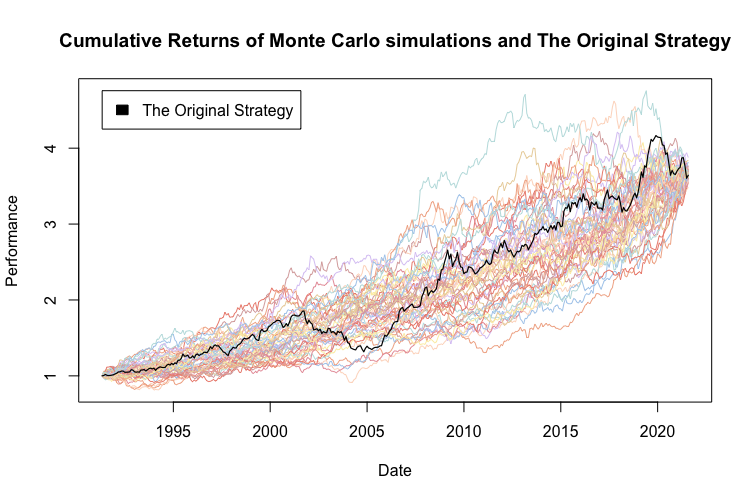
\includegraphics[width=0.6\textwidth]{../Figures/investment_simulation_process.png}
    \caption{Investment Simulation Process for Monte Carlo Analysis}
    \label{fig:investment_simulation}
\end{figure}

\newpage
